\subsubsection{Ekstraksi Data Smart Contracts dari Blockchain Ethereum}

\begin{figure}[ht]
	\centering
	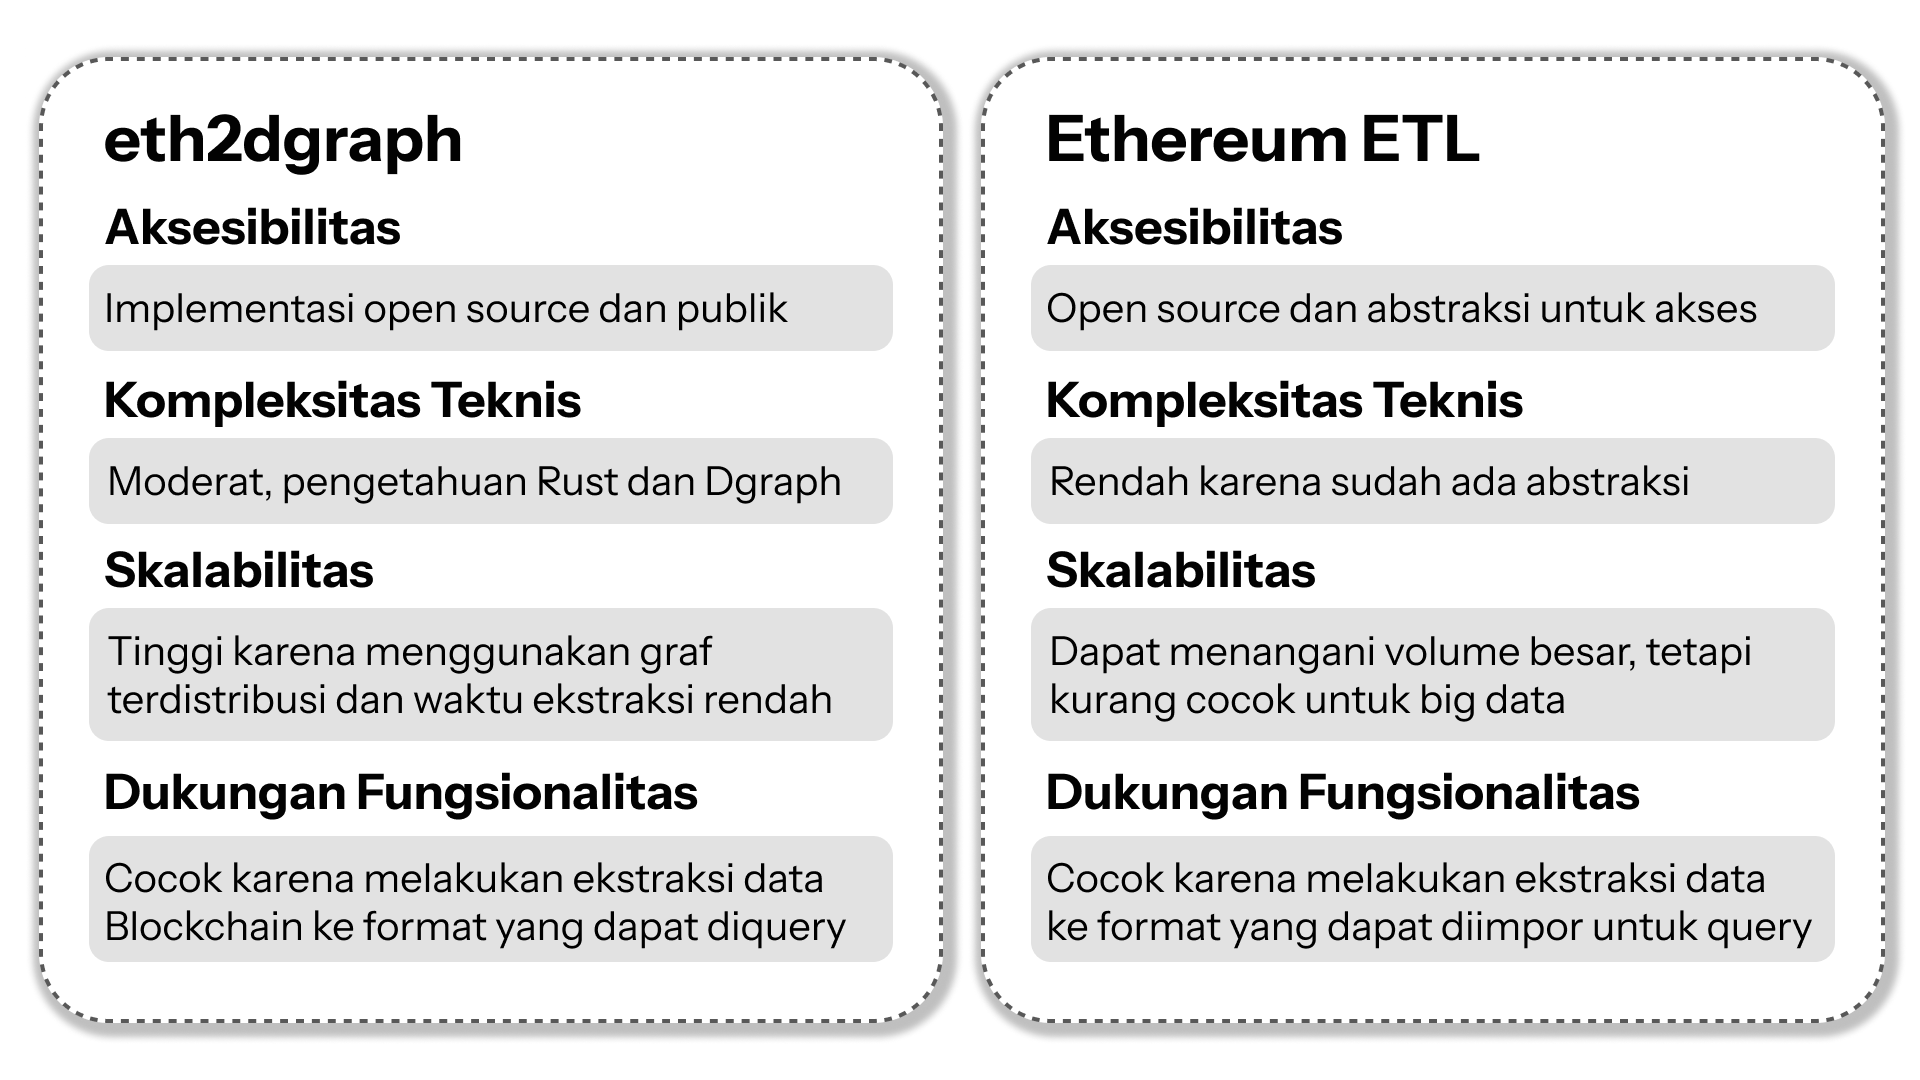
\includegraphics[width=0.9\textwidth]{resources/chapter-3/ekstraksi-1.png}
	\caption{Perbandingan alternatif ekstraksi data Smart Contracts dari Blockchain Ethereum}
	\label{image:perbandingan-ekstraksi-1}
\end{figure}

\begin{figure}[ht]
	\centering
	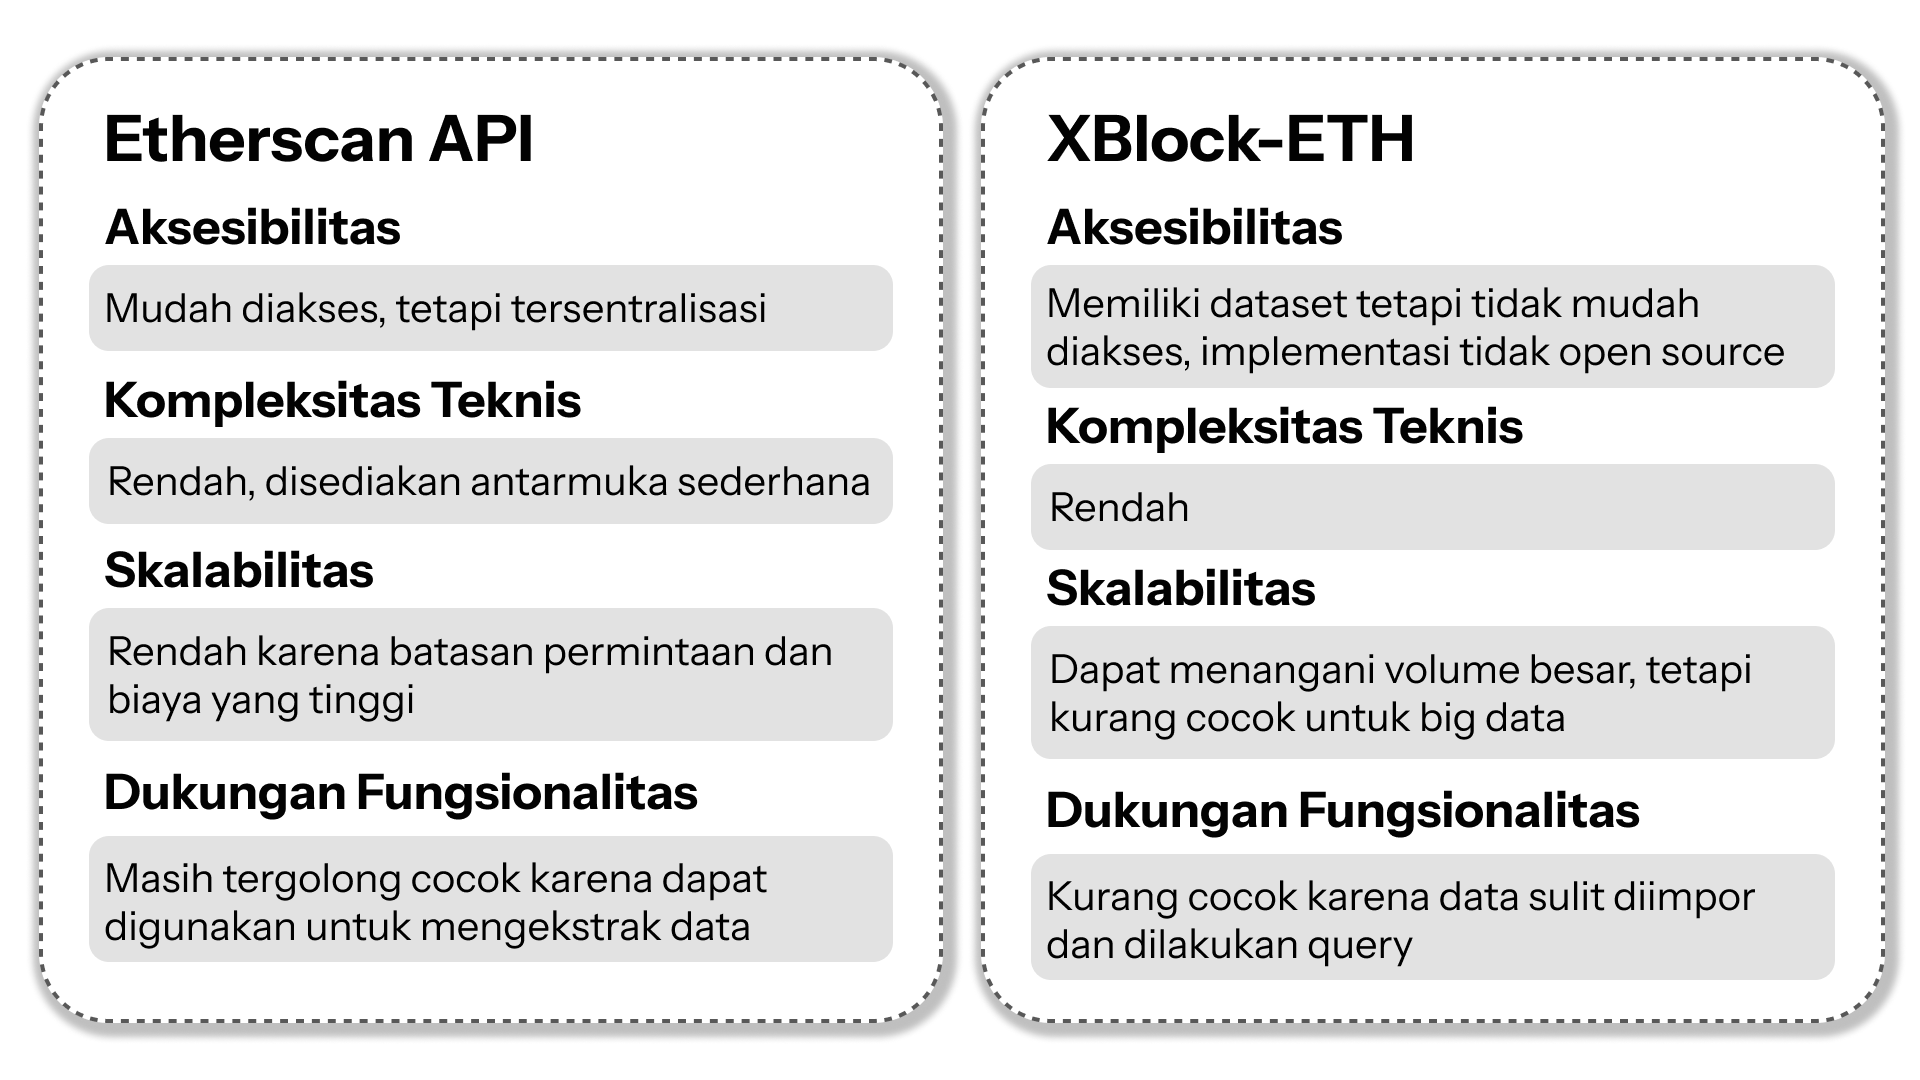
\includegraphics[width=0.9\textwidth]{resources/chapter-3/ekstraksi-2.png}
	\caption{Perbandingan alternatif ekstraksi data Smart Contracts dari Blockchain Ethereum}
	\label{image:perbandingan-ekstraksi-2}
\end{figure}

\begin{figure}[ht]
	\centering
	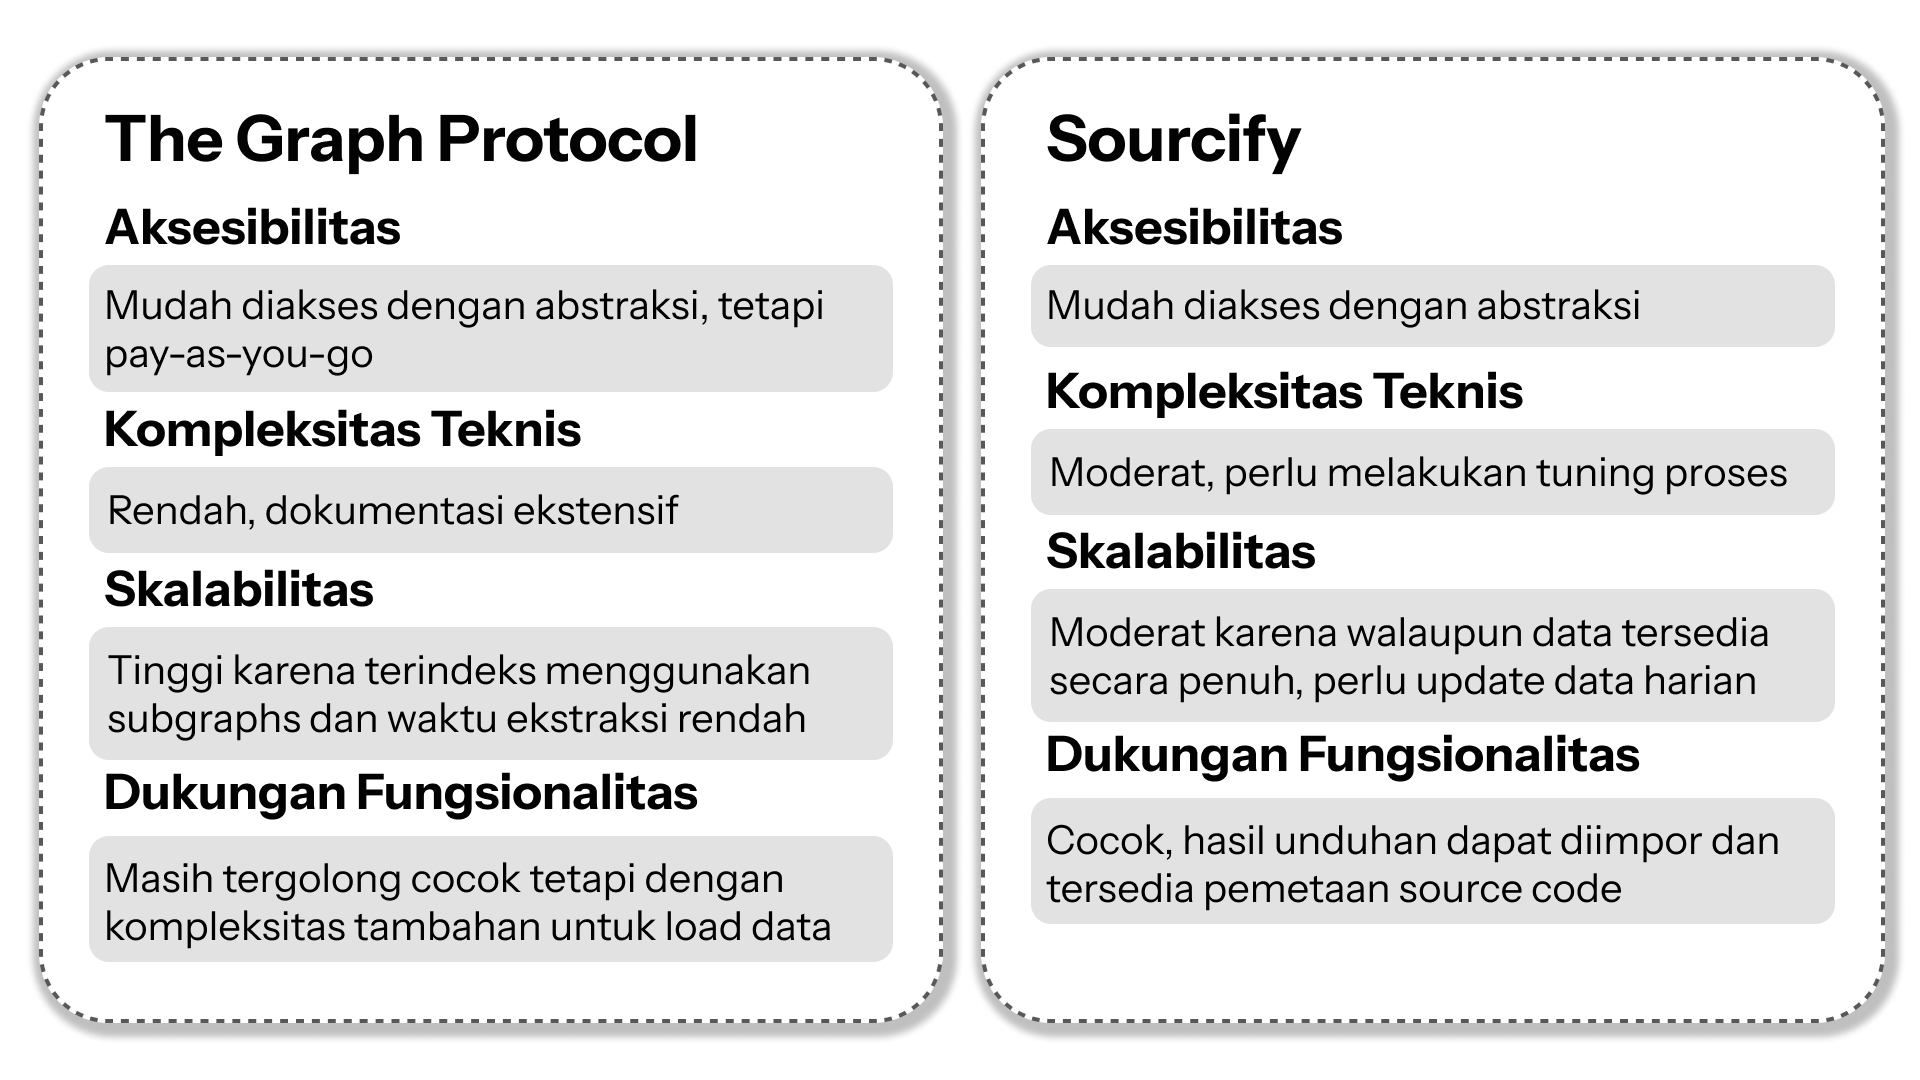
\includegraphics[width=0.9\textwidth]{resources/chapter-3/ekstraksi-3.png}
	\caption{Perbandingan alternatif ekstraksi data Smart Contracts dari Blockchain Ethereum}
	\label{image:perbandingan-ekstraksi-3}
\end{figure}

Kebutuhan pertama yang harus dipenuhi adalah ekstraksi data Smart Contracts dari Blockchain Ethereum. Proses ini mencakup pengambilan data terkait Smart Contracts, seperti ABI, bytecode, metadata, dan Verified \textit{source code}. Data ini akan digunakan untuk membangun basis data yang dapat di-query dan dianalisis lebih lanjut.

Dukungan fungsional yang diperlukan tidak hanya mencakup ekstraksi data, tetapi juga kemampuan memperoleh source code yang terverifikasi dan memetakan source code tersebut dengan deployment untuk analisis tanpa dekompilasi. Prioritas fungsionalnya adalah menghasilkan data dalam format siap pakai, memperoleh source code, dan mengaitkannya dengan deployment. 

Gambar \ref{image:perbandingan-ekstraksi-1}, \ref{image:perbandingan-ekstraksi-2}, dan \ref{image:perbandingan-ekstraksi-3} menunjukkan rangkuman perbandingan berbagai alternatif ekstraksi data Smart Contracts dari Blockchain Ethereum. Secara rinci, berikut adalah analisis dari masing-masing alternatif:

\begin{enumerate}
	\item \textbf{eth2dgraph} \parencite{aimar2023extraction}: Riset ini unggul dalam mengekstrak ABI, bytecode, dan metadata yang dikonversi menjadi format graf. Implementasinya yang \textit{open source} menggunakan Rust untuk kinerja tinggi dan Dgraph untuk skalabilitas, sehingga memungkinkan query pada hubungan antar Smart Contracts di Ethereum. Pendekatan ini memerlukan \textit{node} Ethereum dan dasar pengetahuan mengenai Rust dan Dgraph. Selain ekstraksi cepat, eth2dgraph efektif dalam mengaitkan Smart Contracts Deployment dengan Verified \textit{source code} serta dapat diperluas untuk menambahkan aspek semantik.

	\item \textbf{Ethereum ETL} \parencite{ethereum_etl}: Ethereum ETL dikenal karena kemudahan penggunaan dan dokumentasinya yang lengkap, serta dukungan untuk data transaksi, blok, dan Smart Contracts. Meskipun demikian, ia tidak mendukung ekstraksi ABI, membutuhkan waktu lebih lama, dan memerlukan beberapa operasi tambahan untuk memperoleh data Smart Contracts. Hasil ekstraksinya cocok untuk basis data relasional, namun kurang ideal untuk sistem big data karena format data yang dihasilkan.

	\item \textbf{Etherscan API} \parencite{etherscan2024}: Dengan Etherscan API, pengguna dapat langsung mengekstrak data Smart Contracts beserta Verified \textit{source code} dari sumber yang terpercaya. Antarmukanya yang sederhana memudahkan akses, namun seluruh data bergantung pada Etherscan yang tersentralisasi. Batasan jumlah permintaan serta biaya penggunaan juga perlu diperhitungkan, terutama untuk ekstraksi data skala besar.

	\item \textbf{XBlock-ETH} \parencite{zheng2020xblock}: XBlock-ETH memungkinkan ekstraksi data tanpa memanfaatkan \textit{node} Ethereum, namun hasilnya disimpan dalam bentuk CSV yang memerlukan parsing tambahan dan tidak mendukung query atau indexing secara efisien. Selain itu, karena kode ekstraksinya tidak \textit{open source}, replikasi proses menjadi sulit meskipun pendekatannya cukup sederhana untuk digunakan.

	\item \textbf{The Graph Protocol} \parencite{TheGraphDocs}: The Graph menawarkan kemudahan penggunaan dengan query cepat dan infrastruktur yang terintegrasi dengan baik. Namun, model pembayaran \textit{pay-as-you-go} dapat membuat biaya ekstraksi data meningkat. Data JSON yang dihasilkan memerlukan konversi ulang ke format lain, meski flexibelnya memudahkan pengembangan lebih lanjut.

	\item \textbf{Sourcify} \parencite{sourcify_website}: Sourcify menyediakan antarmuka yang mudah untuk mengunduh dan memetakan hubungan antara \textit{source code} dan Deployment. Meskipun sudah tersedia abstraksi, ia tidak mendukung ekstraksi data kompleks seperti ABI dan bytecode. Proses pengunduhan berkala untuk memperbarui data masih perlu dioptimalkan agar lebih efisien, meskipun penggunaannya tergolong moderat.
\end{enumerate}
